\documentclass[runningheads]{llncs}
\usepackage[T1]{fontenc}
\usepackage{lmodern}
\usepackage{graphicx}
\usepackage{amsmath,amssymb}
\usepackage{booktabs}
\usepackage{array}
\usepackage{adjustbox}
\usepackage{placeins}
\usepackage{multirow}
\usepackage{tikz}
\usetikzlibrary{arrows.meta,positioning,fit}
\usepackage{microtype}
\usepackage[hidelinks]{hyperref}
\renewcommand\UrlFont{\rmfamily}
\makeatletter\newcommand{\inputtab}[1]{\@@input #1 }\makeatother % primitive input: no \relax before \bottomrule
\newcommand{\pmstd}[1]{{\scriptsize$\pm$#1}}
\InputIfFileExists{gen/macros.tex}{}{} % every number quoted in the text, generated from paper_results/
\InputIfFileExists{gen/macros_frontier.tex}{}{} % numbers of the frontier figure (gen/frontier_points.csv)

\begin{document}
\title{Foundation Models and Natural Benchmarks for Image Vertical Federated Learning: When Is One Upload Enough?}
\titlerunning{Foundation models and natural benchmarks for image VFL}
\author{Xavier Desprez\inst{1} \and Oudom Kem\inst{2}}
\authorrunning{X. Desprez and O. Kem}
\institute{\email{xav.desprez@gmail.com}
\and Universit\'e Paris-Saclay, CEA, List, F-91120 Palaiseau, France\\
\email{oudom.kem@cea.fr}}
\maketitle

\begin{abstract}
Vertical federated learning (VFL) lets organisations that hold different features of the same entities train a joint model without pooling their data; with images, for example, satellites operated by different organisations observe the same areas, or different clinics hold complementary images of the same skin lesion. The standard method, split learning, exchanges activations and gradients at every mini-batch, so every party must stay online for thousands of messages. FedOnce needs a single upload, but each party must first train its own encoder on its own, often small, data. We make two contributions. (C1)~We revisit FedOnce with public foundation models: each party encodes its images with a frozen pre-trained encoder, optionally compresses the features with its own PCA, and uploads them once; the label owner then trains the classifier alone. Under one accounting of bytes, messages, party compute and what the label owner sees, we compare this protocol with split learning, logit exchanges, differential privacy and encrypted training. It is the best default: on VertiBench Satellite, \frVbReachSplitNNFoundBytes{} per sample match the accuracy of split learning, which exchanges \frVbReachSplitNNFoundRatio{} times more, and adapting the encoder by split learning gains a few points only on dermatology images, at the price of keeping every party online. (C2)~We assemble benchmarks whose parties hold genuinely different views of the same entity rather than pieces of one image: VertiBench Satellite, reproduced and audited, and a more realistic variant built from the same WorldStrat source, whose two parties hold different sensors and whose folds are grouped by site; and MILK10k, which pairs a clinical and a dermoscopic photograph of each lesion.
\keywords{Vertical federated learning \and Foundation models \and One-shot learning \and Benchmarks \and Communication efficiency \and Privacy}
\end{abstract}

\section{Introduction}\label{sec:intro}

Vertical federated learning (VFL) lets organisations that hold different views of the same entities train a joint model without pooling their raw data~\cite{liu2024vfl}. For images the setting is natural---different satellites, sensors or agencies observe the same locations---yet open benchmarks and methods remain scarce, and the standard training scheme, split learning~\cite{vepakomma2018splitnn}, is expensive: every party exchanges activations and gradients with the label owner at every mini-batch, for every epoch.

A radical alternative is \emph{one-shot} VFL~\cite{wu2022fedonce}: each party computes a representation of its data, uploads it once, and the label owner trains the rest locally. Its weak point is the representation: FedOnce asks every party to run self-supervised pre-training on its own, often small, dataset. Pre-trained vision foundation models~\cite{oquab2024dinov2} offer a different route: the \emph{same frozen encoder} can be shipped to every party, which only needs a forward pass. This idea was prototyped during a research internship at CEA-LIST on satellite images, with a promising headline number; this paper turns the prototype into a systematic study and answers the questions that a deployment would raise:

\begin{itemize}
\item \textbf{Does it work, and why?} We compare, on the public VertiBench satellite benchmark and under one common head/protocol, frozen DINOv2 of four sizes, CLIP, a supervised ImageNet ResNet-50, a randomly initialised ViT, and (for the baselines) end-to-end SplitNN and FedOnce-style SimCLR trained on the raw 13-band images (Sec.~\ref{sec:exp-main}).
\item \textbf{How little needs to be sent?} Per-party PCA and scalar quantisation, fitted without any collaboration, give an accuracy-versus-bytes frontier that goes well below the 96\,KiB per sample of the plain upload (Sec.~\ref{sec:exp-pareto}).
\item \textbf{What if parties are missing, or fewer?} We measure the accuracy as a function of the number of parties and of parties missing at inference, with and without party-level dropout during training (Sec.~\ref{sec:exp-parties}).
\item \textbf{What does the upload leak?} We train feature-inversion decoders against each upload format and relate reconstruction quality to accuracy, bytes and Gaussian noise, and we state why a formal privacy guarantee is out of reach at useful accuracy (Sec.~\ref{sec:exp-privacy}).
\item \textbf{Is the benchmark telling the truth?} On a two-sensor WorldStrat benchmark, a random split lets a location-only model compete with image models; we introduce a geographically disjoint protocol and a selection-free one-shot fusion (Sec.~\ref{sec:exp-ws}).
\end{itemize}

We also correct the preliminary version of this work: its WorldStrat numbers (near-perfect accuracy on the two-sensor task) are not reproduced by the leakage-free, POI-grouped protocol used here and should be disregarded; we report \emph{only} the corrected protocol.

\section{Related Work}\label{sec:related}

\paragraph{VFL and its communication.}
In VFL several parties hold different features of the same samples and one of them holds the labels~\cite{liu2024vfl}. Split learning~\cite{vepakomma2018splitnn} exchanges bottom activations and their gradients at every mini-batch. Communication is reduced by local updates (FedBCD~\cite{liu2022fedbcd}), compressed embeddings (C-VFL~\cite{castiglia2022cvfl}), ADMM-based training (VIMADMM~\cite{xie2024vimadmm}) or the use of non-overlapping samples~\cite{kang2022fedcvt}. One-shot VFL goes further. In FedOnce~\cite{wu2022fedonce} every passive party learns a representation without labels (Noise As Targets~\cite{bojanowski2017nat}) and uploads it once, and Sun et al.~\cite{sun2023oneshotvfl} need three messages and semi-supervised learning to cope with few aligned samples. FeT~\cite{wu2024fet} and LASER-VFL~\cite{valdeira2025laser} relax the alignment and participation assumptions that we keep. VFLAIR~\cite{zou2024vflair} and VertiBench~\cite{wu2024vertibench} make methods comparable, but their image tasks are mostly built by cutting one image into pieces or rendering views of an object~\cite{wu2015modelnet,su2015mvcnn}. VertiBench Satellite, derived from WorldStrat~\cite{cornebise2022worldstrat}, is one of the few with naturally distinct parties, and \cite{wu2025vflpractice} discusses the gap between benchmarks and practice.

\paragraph{Foundation models in federated learning.}
Pre-training matters in \emph{horizontal} federated learning~\cite{nguyen2023where}, where pre-trained backbones are hard to beat~\cite{hu2023flimages}. Training only the last layer on frozen features~\cite{legate2023guiding}, or sharing class-conditional summaries of foundation-model features in a single round (FedPFT~\cite{beitollahi2024fedpft}), removes most of the training and communication. Such summaries need labels at every client, which the passive parties of VFL do not have. Frozen foundation models as VFL party encoders appear in recent work. Split-MoPE~\cite{irureta2026splitmope} uploads frozen DINOv2 embeddings once and trains a mixture of experts that tolerates missing parties. VAFL~\cite{huang2026vafl} fits closed-form heads on frozen ViT features under additively homomorphic encryption, and Jin et al.~\cite{jin2026secure} train on secret-shared frozen ResNet features in a three-server MPC protocol. All three evaluate on patch-split CIFAR-like images. We compare the regimes on naturally partitioned data against reproduced VFL baselines, and we measure the price of freezing, the cost of each regime and the exposure of the upload. The encoders are general vision models (DINOv2~\cite{oquab2024dinov2}, CLIP~\cite{radford2021clip}, SigLIP~\cite{zhai2023siglip}) and domain models for Earth observation (SSL4EO-S12~\cite{wang2023ssl4eo}) and dermatology (BiomedCLIP~\cite{zhang2023biomedclip}, MONET~\cite{kim2024monet}).

\paragraph{Leakage of representations and encrypted training.}
Images can be reconstructed from their features~\cite{mahendran2015understanding,dosovitskiy2016inverting}, with generative decoders even from self-supervised and CLIP embeddings~\cite{bordes2022rcdm,ramesh2022unclip,zheng2026rae,lei2025drag}, and from the activations of collaborative inference~\cite{he2019modelinversion}. VFL is also exposed to data, feature, label and hijacking attacks~\cite{jin2021cafe,luo2021feature,fu2022label,li2022labelleakage,pasquini2021unleashing}. Formal protection comes from differential privacy~\cite{dwork2014algorithmic,dong2022gdp} or from cryptography. Linear and logistic models can be trained on vertically partitioned data with additively homomorphic encryption~\cite{hardy2017private} or secure computation of the Gram matrix~\cite{gascon2017privacy}. They can also be trained on data encrypted once with approximate homomorphic encryption (CKKS) without further interaction~\cite{kim2018logistic,han2019logistic}, with threshold keys when several parties encrypt~\cite{mouchet2021multiparty}. HETAL~\cite{lee2023hetal} trains a softmax head on encrypted foundation-model embeddings with a single data owner. Because these protocols are mature only for linear models, we measure what a linear head costs on frozen features, and what its encrypted training costs.

\section{Operating Regimes and Cost Accounting}\label{sec:method}

\paragraph{Setting and threat model.}
$K$ parties $P_1,\dots,P_K$ hold different images $x_i^{(k)}$ of the same $N$ entities $i$ (an area, a lesion), aligned beforehand, e.g.\ by private set intersection. The label owner, which we call the \emph{server}, holds the labels $y_i$ and may also be a party. Raw images never leave their owner, and the encoder $f$ is public. The server is honest but curious: it follows the protocol and tries to infer the parties' images, or to link uploads to images. It knows $f$, may hold public images of the domain and, in the worst case, copies of candidate images. Malicious parties and label leakage to the parties are out of scope.

\paragraph{R1: one upload of frozen features.}\phantomsection\label{sec:r1}
Each party computes $z_i^{(k)}=f(x_i^{(k)})\in\mathbb{R}^{d}$, the pooled output token of a frozen encoder ($d=768$ for ViT-B, $1024$ for CLIP ViT-L/14~\cite{radford2021clip}, $1536$ for DINOv2 ViT-g/14~\cite{oquab2024dinov2}), averages it over the images it holds of an entity (revisits, or rotated copies of a photograph), and sends it \emph{once}. The server trains a head on the concatenation $[z_i^{(1)};\dots;z_i^{(K)}]$, for as many epochs as it wants, without further communication. Our reference head is a two-layer MLP ($Kd\!\to\!1000\!\to\!C$, batch normalisation, ReLU); on MILK10k, \emph{late fusion} trains one MLP per party and averages their log-probabilities with a weight chosen on validation. \emph{Local compression:} because the encoder is frozen, each party can fit a PCA on its own training features, keep $d'$ components and quantise every coordinate uniformly to $b$ bits between its 1st and 99th training percentiles; the head is trained on the de-quantised values. This needs no labels, no shared basis and no coordination, since the basis stays with the party and the server only needs to know which block comes from which party. The samples must still be aligned, and the per-party bases are mutually incompatible, which matters when parties go missing (Sec.~\ref{sec:frontier-enc}).

\paragraph{R2: a few-round head on frozen features.}
Each party trains a small MLP that maps its frozen features to $C$ logits, and the server sums the logits of all parties. At every training step the parties send the logits of the mini-batch and receive their gradients, i.e.\ $C$ numbers per party and sample in each direction instead of an embedding. The server never receives an embedding.

\paragraph{R3: split learning that adapts the backbone.}
The bottoms are ViT-B backbones that are either frozen (only the top model learns, from activations recomputed on augmented images), adapted with LoRA~\cite{hu2022lora} (rank 16 on the attention query and value projections), or fully fine-tuned. Activations go up and gradients come down at every mini-batch. ResNet-18 bottoms trained from scratch or from ImageNet weights are the non-foundation references.

\paragraph{R4: a linear head trained under encryption.}
After a local PCA to $d'$ components and standardisation, the server fits a ridge classifier $W=(X^\top X+\lambda I)^{-1}X^\top Y$ on one-hot targets. Every party encrypts its feature columns once with CKKS under a threshold key generated jointly by the parties~\cite{mouchet2021multiparty}, so that no single party can decrypt the others' uploads. The server computes the cross-party blocks $X_k^\top X_l$ and $X_k^\top Y$ homomorphically, masks them, has them decrypted collectively and solves the system in the clear. This takes one upload and one round trip of $\mathcal{O}(D^2)$ aggregates, with $D=Kd'$. No per-sample vector is ever decrypted, but the server learns the second-order statistics $X^\top X$ and $X^\top Y$, as in other closed-form protocols~\cite{gascon2017privacy,huang2026vafl}, and the trained model. $\lambda$ is chosen from validation scores, obtained by applying each candidate model to encrypted validation uploads and decrypting only the scores. Class weights and the encrypted alternative, logistic regression with bootstrapping~\cite{kim2018logistic,han2019logistic}, are discussed in App.~\ref{app:privacy}. We emulate the ridge in plaintext (CKKS adds a relative error of the order of $10^{-6}$, which we measure) and time its homomorphic operations with a single key in TenSEAL. The threshold key generation and the collective decryption are not timed.

\paragraph{Cost accounting.}\phantomsection\label{sec:accounting}
We count four costs, analytically and per aligned training sample. (i)~\emph{Bytes:} the cumulative payload of a whole training run, summed over all parties and both directions, in half precision. R1 costs $Kd'b/8$ bytes once (b=16 without quantisation), independently of the number of epochs and of re-trainings. Split learning costs $4Kd_{\mathrm{act}}$ bytes per epoch, for activations up and gradients down, or half of that with frozen bottoms; R2 costs $4KC$ bytes per epoch. Downloading the public encoder, quantiser bounds and inference (one vector or activation per party and entity in every regime) are not counted. (ii)~\emph{Rounds:} the synchronised exchanges during training, i.e.\ one for R1, one per mini-batch for R2 and R3, and one upload plus one round trip of aggregates for R4. (iii)~\emph{Party compute:} forward GFLOPs per image, where a training step costs about three forward passes. In R1, R2 and R4 a party runs one forward pass per image and no backpropagation, and the features can be cached and reused. This is not the least compute: one DINOv2-g pass costs \vbGGF{} GFLOPs per image, more than the \rEighteenTrainGF{} GFLOPs of 50 training epochs of the ResNet-18 bottom of the VertiBench reference. (iv)~\emph{Server view:} per-sample embeddings (or their PCA codes) in R1, per-sample logits during training in R2, per-sample activations in R3, and aggregates in R4.

\section{Natural Benchmarks for Image VFL}\label{sec:setup}

Our second contribution is a set of image VFL benchmarks with naturally distinct parties and an evaluation protocol (Table~\ref{tab:bench}). Natural parties see the same entity through different sensors, dates or devices, whereas split benchmarks create complementarity by cutting one image. On MILK10k, cutting the dermoscopy into two halves even \emph{loses} information (\milkGHalves{} against \milkGDerm\,\% macro F1 for the whole image, DINOv2-g), because each party's encoder sees half a lesion.

\begin{table}[t]
\caption{The benchmarks. $K$: parties; $N$: aligned entities; $C$: classes. WorldStrat and the classic splits are detailed in App.~\ref{app:ws} and~\ref{app:classic}.}\label{tab:bench}
\centering\scriptsize
\setlength{\tabcolsep}{2.5pt}
\begin{tabular}{@{}p{1.7cm}cp{2.55cm}rcp{1.55cm}p{3.4cm}@{}}
\toprule
Benchmark & $K$ & Each party holds & $N$ & $C$ & Metric, folds & Audit / key finding\\
\midrule
VertiBench Satellite~\cite{wu2024vertibench} & 16 & one Sentinel-2 revisit of the area (13 bands) & 3{,}927 & 4 & accuracy; official split, 5 seeds & reference reproduced; \auSibShare\,\% of test tiles have a training tile of the same site, confounded with class\\
MILK10k~\cite{milk10k} & 2 (+1) & a clinical or a dermoscopic photograph of the lesion (+ metadata) & \milkN & 7 & macro F1; 5 folds over lesions & the photographs fail on the same lesions; cutting one image into halves loses F1\\
WorldStrat, two sensors (ours)~\cite{cornebise2022worldstrat} & 2 & a 1.5\,m SPOT image, or 16 Sentinel-2 revisits & \wsIpccN & 7, 18, 8 & macro F1; 5 site-grouped folds & stratified folds overstate F1 by 6--9 points; the second sensor adds little\\
\midrule
Split CIFAR, ModelNet40 & 2--12 & a piece of one image, or rendered views & -- & 10--100 & accuracy; official splits & gains over published methods mostly measure pre-training\\
\bottomrule
\end{tabular}
\end{table}

\paragraph{VertiBench Satellite, reproduced and audited.}\phantomsection\label{sec:vb-audit}
Each of the 16 parties holds one Sentinel-2 L1C revisit ($158\times158$ pixels, 13 bands) of 3{,}927 areas, labelled by their sampling source (majority class: \majVB\,\%). We keep the official split (3{,}142 training and \giVbNTest{} test samples) and hold out 15\,\% of the training samples for validation. The parties see the same sensor at different dates and are largely redundant: one party alone gives \soloMean\,\% accuracy on average, all 16 give \partiesKAll\,\%. Our re-implementation of the published split-learning reference reaches $\reproAcc\pm\reproStd$\,\%, in line with the published value (Table~\ref{tab:main}). Image fingerprints map \auMapTrain{} training and \auMapTest{} test samples to distinct source areas, none in both splits. However, \auSibN{} test samples (\auSibShare\,\%) have a training tile of the same site, all in the two classes whose sites are cut into $3\times3$ tiles, so sibling and class effects are confounded. The reproduced SplitNN is more accurate on these samples (\auSnSib{} vs.\ \auSnNoSib\,\%), the CLIP-L one-shot head is not (\auClipSib{} vs.\ \auClipNoSib\,\%); we keep the official split and also report the subset without siblings (App.~\ref{app:audit}).

\paragraph{MILK10k: two photographs of the same lesion.}
MILK10k~\cite{milk10k} pairs, for \milkN{} lesions, a clinical close-up (party~A, e.g.\ the referring practitioner) and a dermoscopic image (party~B, the dermatologist), with metadata (optional party~C) and a confirmed diagnosis, which we group into 7 classes. Without patient identifiers, the five stratified folds are drawn over lesions. With only 40 to 61 lesions of the two rarest classes per test fold, macro F1 is the metric and comparisons are paired by fold. The two parties are wrong together on \mfGBoth\,\% of the lesions, against \mfGIndep\,\% if their errors were independent (App.~\ref{app:milk}).

\paragraph{WorldStrat: two sensors.}
From WorldStrat~\cite{cornebise2022worldstrat} we build a two-party task on \wsIpccN{} areas of $1.58\times1.58$\,km: a pan-sharpened 1.5\,m SPOT image (party~A) and 16 Sentinel-2 revisits (party~B), with three labels read at the centre of the area: land cover~\cite{esa2017cci} (18 classes), its IPCC category (7) and the degree of urbanisation~\cite{pesaresi2019ghsl} (8). Stratified folds put neighbouring tiles of a site in training and test and overstate macro F1 by about 6 to 9 points on land cover, so folds are grouped by site. Adding the Sentinel-2 party to SPOT then changes macro F1 by \wgIpccA{} points on IPCC (\wgIpccAW{} folds improve), \wgLccsA{} on land cover (\wgLccsAW) and \wgSmodA{} on urbanisation (\wgSmodAW): the second sensor adds little, so this benchmark tests fusion rather than the frontier (App.~\ref{app:ws}).

\paragraph{Protocol.}
Costs are counted as in Sec.~\ref{sec:accounting}. \emph{Baselines} trained on raw images: the reproduced VertiBench SplitNN (one ResNet-18 per party, 13 bands, 50 epochs, last epoch tested); our split-learning recipe with ResNet-18 bottoms~\cite{he2016resnet} from scratch or ImageNet weights; FedOnce~\cite{wu2022fedonce} with Noise As Targets~\cite{bojanowski2017nat} or SimCLR~\cite{chen2020simclr} pre-training by each party; and R3 with ViT-B bottoms for 10 epochs with augmentation. None was tuned extensively. \emph{Encoders} are used through their pooled token at 224\,px, with satellite images standardised per band and fed as RGB (list in App.~\ref{app:vb}). CLIP ViT-L/14 is the main VertiBench encoder, as the most accurate single encoder and one with a public generative decoder; DINOv2 ViT-g/14, with the largest $d$, serves for the compression grid, missing parties and the MILK10k reference; adapted backbones are ViT-B (CLIP ViT-B/16, DINOv2 ViT-B/14), always compared with the same ViT-B frozen. \emph{Heads} use Adam, early stopping on the validation loss and, on MILK10k and WorldStrat, a class-balanced loss. \emph{Statistics:} on VertiBench, mean\,$\pm$\,std over five seeds on the fixed test set (three for ViT split learning) and paired comparisons with the reproduced SplitNN on the same test predictions (probabilities averaged over three seeds; exact McNemar test, paired bootstrap intervals); on MILK10k and WorldStrat, five folds, paired by fold.

\section{The Accuracy--Cost Frontier}\label{sec:frontier}

Figure~\ref{fig:frontier} places every method we run on the two main benchmarks by its training payload per sample and its score. On both, the envelope consists of foundation-encoder points only (\frVbNParetoFound{} of \frVbNPareto{} points on VertiBench, \frMilkNParetoFound{} of \frMilkNPareto{} on MILK10k); which regime lies on it depends on the budget and the domain. We claim a default, not strict domination: on party compute alone, a frozen ImageNet ResNet-50 (8 GFLOPs per image, 80.9\,\%) is cheaper than every foundation encoder we test, an exception that does not change the default.

\begin{figure}[t]
\centering\IfFileExists{gen/fig_frontier.pdf}{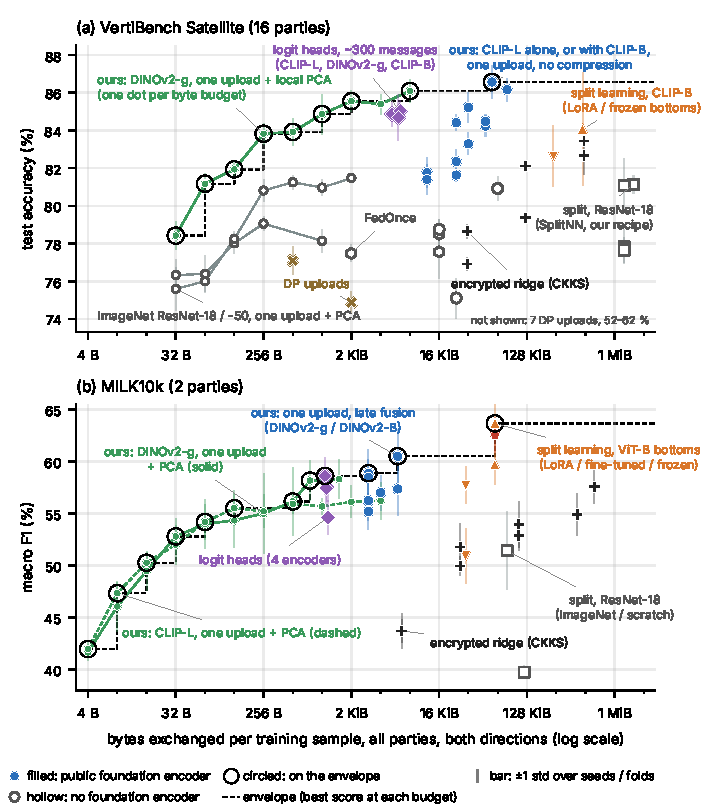
\includegraphics[width=0.92\linewidth]{gen/fig_frontier.pdf}}{\fbox{\parbox{0.9\linewidth}{\centering fig\_frontier pending}}}
\caption{The accuracy--communication frontier on VertiBench Satellite (left) and MILK10k (right). Horizontal axis: bytes exchanged per training sample over a training run, all parties and both directions (for the encrypted heads, the encrypted upload only). Filled markers use a foundation encoder, hollow ones do not; bars: std over seeds or folds; circled: envelope. VertiBench PCA points are selected on validation at each budget; seven DP points (\dpFullOne--\dpStEight\,\%) lie below the axis.}\label{fig:frontier}
\end{figure}

\subsection{VertiBench: one compressed upload is the knee}\label{sec:frontier-vb}\phantomsection\label{sec:exp-main}

\begin{table}[t]
\caption{VertiBench Satellite (16 parties, official test set). Upload: training payload per sample over all parties (activations or logits up, gradients down when needed). GFLOPs: party compute per image (a training run for split learning, one forward pass otherwise). Time: minutes on one A100 (split training, FedOnce pre-training or feature extraction). Mean\,$\pm$\,std over 5 seeds unless noted; --: not recorded.}\label{tab:main}
\centering\scriptsize
\setlength{\tabcolsep}{3pt}
\begin{adjustbox}{max width=\linewidth}
\begin{tabular}{@{}lcrrrccc@{}}
\toprule
Method & Bands & Upload & GFLOPs & Time & Acc. (\%) & F1 (\%) & AUC (\%)\\
\midrule
\inputtab{gen/tab_main.tex}
\bottomrule
\end{tabular}
\end{adjustbox}
\end{table}

\paragraph{No trained or split-learning point is on the envelope.}
Our split-learning recipe matches the reproduced reference only from ImageNet weights (\splitPTAcc\,\%), and FedOnce, whose parties pre-train their own encoders, reaches \natAcc{} to \sslAllAcc\,\% (Table~\ref{tab:main}). The best non-foundation point, the reproduced SplitNN (\frVbBestNonFound\,\% for \frVbBestNonFoundBytes{} over 50 synchronised epochs), is matched by one upload of \frVbBeatNonFoundBytes{} per sample (\frVbBeatNonFoundName: \frVbBeatNonFound\,\%), with \frVbBeatNonFoundRatio{} times fewer bytes. The frozen ResNet-50 (80.9\,\% for 64\,KiB) is off the envelope too; we have not compressed its features.
% UPDATE when the ResNet-18/50 + PCA control on VertiBench is available.

\paragraph{One upload.}
Uncompressed, frozen CLIP-L reaches \vbClipAcc\,\% (32\,KiB), DINOv2-g \vbGAcc\,\% and CLIP-B \vbClipBAcc\,\%. Against a three-seed SplitNN re-run (\auSnAll\,\%), CLIP-L gains $\pairSnClipDiff$ points ($[\pairSnClipLo,\pairSnClipHi]$, $p\pairSnClipP$), CLIP-B $\pairSnClipBDiff$ ($p\pairSnClipBP$) and DINOv2-g $\pairSnGDiff$, which is not significant ($[\pairSnGLo,\pairSnGHi]$, $p\pairSnGP$); the four-logit heads give $p\pairSnLgClipP$, $p\pairSnLgGP$ and $p\pairSnLgClipBP$, and LoRA split learning $p\pairSnLoraP$. All eight leads are positive and grow without training siblings (CLIP-L: $\pairSnClipNoSibDiff$ points, $p\pairSnClipNoSibP$), but the $p$-values are uncorrected: a Holm correction leaves only LoRA and the CLIP-B four-logit head below 0.05. The compressed uploads below were not paired-tested.

\paragraph{The PCA knee.}\phantomsection\label{sec:exp-compress}
Selected on validation under a byte budget, DINOv2-g uploads compressed by each party reach \selTwoAcc\,\% at \selTwoBytes{} per sample (all 16 parties), \selTwokAcc\,\% at \selTwokBytes{} (\selTwokCfg) and \selFullAcc\,\% at \selFullBytes, against \fullAcc\,\% uncompressed at 48\,KiB: on few labels, compression also regularises (App.~\ref{app:pca}). Beyond \selTwokBytes, four times more bytes buy half a point, and the most accurate point, two encoders side by side, reaches \frVbBest\,\% at \frVbBestBytes. This standard compression has limits: incompatible per-party bases break a head that averages the parties' vectors (\poolGMean{} to \poolGPcaMean\,\%; Sec.~\ref{sec:frontier-enc}), and on MILK10k PCA slightly lowers macro F1 (\mrGPca{} vs.\ \mrGCat\,\%, DINOv2-g).

\paragraph{Rounds and adaptation do not pay here.}
The four-logit heads reach \lgClipAcc\,\% (CLIP-L), \lgGAcc\,\% (DINOv2-g) and \lgClipBAcc\,\% (CLIP-B) for \lgClipUp--\lgGUp{} over about \lgClipEp{} synchronised epochs, below the \selTwokBytes{} upload; their interest is exposure (Sec.~\ref{sec:server}). Split learning with CLIP-B bottoms reaches \vbSplitLoraAcc\,\% with LoRA (\vbSplitLoraN{} seeds, \vbSplitLoraUp) and \vbSplitFrozenAcc\,\% frozen, against \vbClipBAcc\,\% for one upload of the same encoder: on VertiBench the most accurate points are frozen.

\paragraph{Party compute.}
Without backpropagation, a party computes one cacheable forward pass per image, which is not minimal compute: DINOv2-g costs \vbGGF{} GFLOPs per image, more than the \rEighteenTrainGF{} of training the SplitNN bottom, CLIP-B \vbClipBGF{} and ResNet-50 8. Encoding all images takes \vbGMin{} minutes with DINOv2-g and \vbClipBMin{} with CLIP-B on one A100, against \reproMin{} per SplitNN run\IfFileExists{gen/fig_frontier_axes.pdf}{ (frontier along compute, rounds and exposure: Fig.~\ref{fig:frontier-axes})}{}.

\subsection{MILK10k: the price of freezing}\label{sec:frontier-milk}\phantomsection\label{sec:exp-freeze}

\begin{table}[t]
\caption{The price of freezing on MILK10k (2 parties, 5 folds, class-balanced loss). Split learning trains the bottoms with the server's gradients; one-shot rows use frozen features and an MLP head (concatenation, or late fusion on features averaged over 8 rotations and flips). Upload per training sample: over 10 epochs for split learning, once for one-shot. Time: minutes per fold (one-shot: encoding, estimated).}\label{tab:freeze}
\centering\scriptsize
\setlength{\tabcolsep}{3pt}
\begin{adjustbox}{max width=\linewidth}
\begin{tabular}{@{}llrrrccc@{}}
\toprule
Party models & Training & Trainable & Upload & Time & F1 (\%) & Bal.\ acc.\ (\%) & Acc.\ (\%)\\
\midrule
\inputtab{gen/tab_freeze.tex}
\bottomrule
\end{tabular}
\end{adjustbox}
\end{table}

\paragraph{Adaptation is the accuracy end.}
A \frMilkBeatNonFoundBytes{} upload (\frMilkBeatNonFoundName) already reaches \frMilkBeatNonFound\,\% macro F1, above the best non-foundation point, ImageNet ResNet-18 split learning (\frMilkBestNonFound\,\% for \frMilkBestNonFoundBytes). The envelope continues through multi-view late fusion (\frMilkBestOneShot\,\% for \frMilkBestOneShotBytes) to DINOv2-B with LoRA (\frMilkBest\,\% for \frMilkBestBytes), whose lead is smaller than its fold standard deviation. With the same backbone and head, LoRA raises F1 from \fzdinovTwob{} to \fzdinovTwoblora\,\% (DINOv2-B) and from \fzclipbSixteen{} to \fzclipbSixteenlora\,\% (CLIP-B); full fine-tuning is no better (\fzdinovTwobft\,\%). Freezing thus costs \fzGapCb{} to \fzGapB{} points, but split learning also trains on augmented images: when the frozen parties average the features of 8 rotations and flips and the server fuses per-party heads, the gap shrinks to \fzGapViewsCb--\fzGapViewsB{} points (late fusion beats concatenation on all folds, as expected from modality competition~\cite{wang2020makes,peng2022balanced}; App.~\ref{app:milk}). Under one split-learning recipe, LoRA beats frozen bottoms on all folds ($\srGapB\pm\srGapSdB$ points for DINOv2-B, $\srGapCb\pm\srGapSdCb$ for CLIP-B), but frozen CLIP-B bottoms then shift F1 by $\srVsHeadCb$ points relative to the one-shot head, so part of that gain reflects a weak baseline. These points require every party to backpropagate on a GPU and stay online, exchanging \fzUpdinovTwoblora{} per sample instead of 3\,KiB once. We have not run the four-logit head or DP on MILK10k.
% UPDATE when the MILK10k four-logit and PCA-grid runs are available.

\paragraph{When to adapt.}
Adaptation buys several F1 points on dermatology images and nothing on Sentinel-2 composites, which we attribute to their distance from web-scale pre-training data, a hypothesis two benchmarks cannot establish. Domain encoders do not close the gap: SSL4EO-S12 stays below CLIP-L on VertiBench (Table~\ref{tab:main}), BiomedCLIP and MONET below DINOv2-g on MILK10k (App.~\ref{app:milk}).

\subsection{Encoder choice and missing parties}\label{sec:frontier-enc}
Pre-trained ViTs lie within a few points of each other on VertiBench, a randomly initialised ViT-B reaches 75.1\,\% (App.~\ref{app:vb}), and small encoders (DINOv2-S: \vbDinoSAcc\,\%, \vbDinoSGF{} GFLOPs) suit parties without accelerators. With 12 of 16 parties missing at inference, a concatenation head falls to \missZeroTwelveZ\,\% if missing uploads are zeroed and \missZeroTwelveM\,\% with mean imputation, whereas a head that normalises and averages the vectors of the parties present keeps \poolMissTwelve\,\% (\poolMissFifteen\,\% with one party); it needs a shared feature space, which per-party PCA and distinct modalities remove.

\section{What the Server Sees}\label{sec:server}\phantomsection\label{sec:exp-privacy}

The frontier of Sec.~\ref{sec:frontier} counts bytes, not exposure. On exposure, the regimes form a ladder. (i)~\emph{No formal guarantee:} plaintext or PCA uploads (R1), per-party logits (R2), and split learning (R3), which exposes plaintext activations at every step of every epoch and returns gradients to the parties. (ii)~\emph{A formal but loose guarantee:} Gaussian noise added to the upload by each party. (iii)~\emph{Individual vectors hidden:} the ridge head trained under CKKS (R4), which reveals second-order statistics. Local PCA is what makes levels (ii) and (iii) affordable. In Fig.~\ref{fig:frontier}, the best points at which the server receives no plaintext feature are a DP upload after PCA-16 (\dpStSsf\,\% for 512\,B) and the CLIP-L ridge heads under CKKS (up to \heVbCRidgeTf\,\%). We first measure what level (i) reveals.

\subsection{Plaintext uploads are linkable and partly decodable}

\begin{figure}[t]
\centering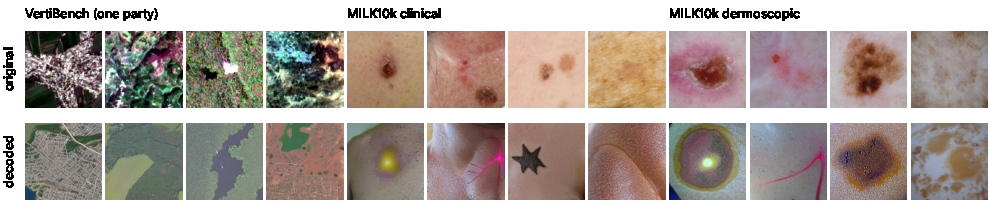
\includegraphics[width=\linewidth]{gen/fig_generic.pdf}
\caption{A public image generator (Stable unCLIP~2.1) applied, without any adaptation, to the CLIP-L uploads of held-out images: the first four attacked test images of VertiBench (one party; contrast-stretched for display) and of MILK10k. It returns an image of the same kind, not the image.}\label{fig:generic}
\end{figure}

\paragraph{Linkage.}
Because the encoder is public, an attacker who holds copies of the candidate images needs no decoder: it encodes them and matches the uploads. Among the \lkN{} VertiBench test images of all parties, the top-1 linkage of CLIP-L uploads is \lkSame\,\% when the attacker reproduces the party's preprocessing, \lkBicubic\,\% after bicubic resizing and \lkEightbit\,\% after 8-bit quantisation, but \lkClip\,\% with CLIP's standard preprocessing. The attack only needs a preprocessing close to the party's.

\paragraph{Decoding.}
Without the images, a public generator decodes part of the content. Stable unCLIP~\cite{ramesh2022unclip,rombach2022ldm}, applied unchanged to VertiBench CLIP-L uploads, returns an image of the same kind of scene, not the image (Fig.~\ref{fig:generic}). An independent encoder (DINOv2-B) picks the source among the \giVbNTest{} test images of the party in \giVbReid\,\% of the cases (top-10: \giVbReidTen\,\%; chance: \giVbChance{} and \giVbChanceTen\,\%). A classifier trained on real images predicts the label from the reconstruction with \giVbLabFone\,\% macro F1, against \giVbRealFone\,\% from the image itself and \giVbChanceFone\,\% by chance. On MILK10k, the decoder draws a lesion-like spot on skin but recovers neither the lesion nor its diagnosis (\giMilkClinLabFone{} and \giMilkDermLabFone\,\% macro F1 for the two modalities, chance \giMilkChanceFone\,\%): what it recovers depends on how well its training images cover the domain. Fine-tuned on public in-domain pairs, the decoder re-identifies no more sources (\giVbBestReid\,\%) and recovers the label only slightly better (\giVbBestLabFone\,\%), while the nearest public image in CLIP space predicts the label as well as the image itself (\giVbNnLabFone\,\%). Decoders trained with a pixel loss on in-domain pairs recover colour, not layout (App.~\ref{app:privacy}). All these attacks bound the leakage from below. We did not attack the pooled DINOv2 token with a generative decoder, nor the activations and features of the trained baselines (SplitNN, FedOnce). Exposure across regimes is therefore compared by what the server receives, not by measured leakage.

\subsection{Party-side transforms and differential privacy}

\paragraph{Secret transforms do not survive a few leaked pairs.}
A party can transform its CLIP-L features before uploading them, with a secret rotation, a private PCA-64, the code of an autoencoder trained on its own features, or a one-layer bottleneck trained by split learning. The attacker then maps the transformed uploads back to CLIP embeddings. Without any image--upload pair of the party, our spectral alignment with public features fails (\gdRotLinkZero\,\% linkage for the rotation). With 100 leaked pairs, i.e.\ 3\,\% of a party's samples, a ridge regression links \gdPcaLinkOneZeroZero{} to \gdAeLinkOneZeroZero\,\% of the uploads for the rotation, the PCA and the autoencoder, and \gdSplitLinkOneZeroZero\,\% for the split bottleneck. Only noise-as-targets codes resist (\gdNatLinkThreeOneFourTwo\,\% with all training pairs), at a cost of \gdNatDrop{} accuracy points (App.~\ref{app:privacy}). A transform that preserves accuracy preserves the information an attacker needs.

\paragraph{Differential privacy is usable after PCA.}
Each party clips its vector, raw or after PCA, at the median norm of its own training vectors and adds isotropic Gaussian noise calibrated to a per-upload $(\varepsilon,\delta{=}10^{-5})$ guarantee by Gaussian DP~\cite{dong2022gdp}. The noise norm grows with the square root of the dimension and the clipped signal does not, so a lower dimension means less noise: PCA is what makes DP usable. At $\varepsilon=8$ per upload, full DINOv2-g features fall to \dpFullEight\,\%, below the majority class (\majVB\,\%), whereas PCA-16 uploads keep \dpStEight\,\%. At $\varepsilon=64$, PCA-16 reaches \dpStSsf\,\% and PCA-64 \dpSfSsf\,\%, against \dpFullSsf\,\% for full features. The guarantee is formal but loose. $\varepsilon$ is per upload, and the 16 uploads of a sample compose to about $\varepsilon\approx50$ for a per-upload $\varepsilon=8$ and $\varepsilon\approx630$ for $\varepsilon=64$, before accounting for the estimation of the clipping norms and of the PCA bases on the training data. The reproduced SplitNN (\reproAcc\,\%) offers no formal guarantee, so DP buys a guarantee, at an accuracy cost.

\subsection{The encrypted point: a ridge head under CKKS}\label{sec:he}

\begin{table}[t]
\caption{Heads that can be trained on encrypted uploads. Accuracy on VertiBench (16 parties) and CIFAR (2 parties), macro F1 on MILK10k and WorldStrat (2 parties); mean\,$\pm$\,std over 5 seeds or folds (CIFAR: 3 seeds). MLP: the reference head, re-run in the same pipeline as the ridge (hence differences of a tenth of a point from Table~\ref{tab:main}). Ridge: closed form from $X^\top X$ and $X^\top Y$ on standardised features (class-weighted on MILK10k and WorldStrat), regularisation chosen on validation, emulated in plaintext; PCA to 256, 64 or 16 components per party; --: Gram matrix too large to emulate (16 parties, full features).}\label{tab:he}
\centering\scriptsize
\setlength{\tabcolsep}{4pt}
\begin{adjustbox}{max width=\linewidth}
\begin{tabular}{@{}lccccc@{}}
\toprule
& \multicolumn{2}{c}{Full features} & \multicolumn{3}{c}{Ridge after per-party PCA}\\
\cmidrule(lr){2-3}\cmidrule(lr){4-6}
Task & MLP & Ridge & 256 & 64 & 16\\
\midrule
\inputtab{gen/tab_he.tex}
\bottomrule
\end{tabular}
\end{adjustbox}
\end{table}

\paragraph{Accuracy.}
With two parties and full features, linearity costs little or nothing on some tasks and a few points on others (Table~\ref{tab:he}): the ridge matches or exceeds the MLP on MILK10k with DINOv2-g (\heMilkGRidgeFull{} vs.\ \heMilkGMlp\,\%) and on WorldStrat IPCC (\heworldstratipccRidgeFull{} vs.\ \heworldstratipccMlp\,\%), but loses on MILK10k with CLIP-L (\heMilkCRidgeFull{} vs.\ \heMilkCMlp\,\%). The encrypted cost, however, grows with the square of the total dimension $D=Kd'$, and 16 full parties are too large even to emulate. After a per-party PCA, the ridge reaches on VertiBench \heVbGRidgeTf{} to \heVbCRidgeTf\,\% with PCA-256, \heVbGRidgeSf{} to \heVbCRidgeSf\,\% with PCA-64 and \heVbGRidgeSt{} to \heVbCRidgeSt\,\% with PCA-16 (DINOv2-g to CLIP-L), against \reproAcc\,\% for plaintext SplitNN. On MILK10k, PCA-64 lowers it to \heMilkGRidgeSf\,\% (DINOv2-g), the level of ResNet-18 split learning from ImageNet weights.

\paragraph{Cost.}
We timed the CKKS operations with TenSEAL on one CPU core (parameters in App.~\ref{app:privacy}). An encrypted inner product of two feature columns takes about \hcVbStCtCt\,ms, and the server needs one per pair of columns from different parties. This amounts to \hcVbStServerH{} core-hours for VertiBench with PCA-16 and \hcVbSfServerH{} with PCA-64. For the class-weighted MILK10k ridge, it amounts to \hcMilkServer{} core-minutes with PCA-64, but about \hcMilkFullH{} core-hours with the full features that its accuracy requires. Encryption also expands each upload \hcVbSfExpand-fold: with PCA-64, a VertiBench party sends \hcVbSfUp{} for its \hcVbSfN{} training samples instead of \hcVbSfPlain{} in half precision, and a MILK10k party with full features sends \hcMilkFullUp. These are operation timings with a single key, and accuracies emulated in plaintext with a measured CKKS error of the order of $10^{-6}$. The collective decryption, the repacking of the aggregates and the end-to-end protocol remain to be implemented. At affordable dimensions, the encrypted ridge therefore scores around or below the plaintext non-foundation reference, and it reveals $X^\top X$ to the server: it is the security end of the frontier, at a cost in accuracy and compute.

\section{Decision Guide and Limitations}\label{sec:discussion}

\paragraph{Which regime under which constraint.}
On our benchmarks, a foundation encoder is the default, and the binding constraint selects the regime:
\begin{itemize}
\item \emph{bandwidth, or parties online only once:} one upload compressed by local PCA (R1); on VertiBench, \selTwokBytes{} per sample for \selTwokAcc\,\%;
\item \emph{accuracy, in a domain far from pre-training:} split learning with LoRA (R3), if every party can train and stay online; \fzGapCb{} to \fzGapB{} F1 points on MILK10k for \fzUpdinovTwoblora{} per sample, nothing on VertiBench;
\item \emph{no embedding at the server, rounds acceptable:} the four-logit head (R2), whose own leakage we did not measure;
\item \emph{a formal guarantee:} DP noise on a PCA upload, loose and at an accuracy cost;
\item \emph{individual vectors hidden:} a ridge head under CKKS on PCA uploads (R4), at a cost in accuracy and compute, and revealing $X^\top X$.
\end{itemize}
Secret transforms are no substitute, and plaintext uploads are linkable whenever the server may hold the images.

\paragraph{Limitations.}
The frontier is the envelope of the methods we ran, on two main benchmarks of one domain each, with untuned baselines; a compressed frozen ImageNet encoder was not tested, nor were the four-logit head and DP on MILK10k. VertiBench parties are redundant and its sibling tiles confounded with class; the paired tests use three seeds and are uncorrected. MILK10k lacks patient identifiers, and its freezing gaps depend on the recipe. Alignment is assumed complete. The attacks are lower bounds, and the encrypted head is emulated.
% UPDATE: drop the ImageNet-encoder and MILK10k clauses when chain F is in.

\section{Conclusion}\label{sec:conclusion}
We asked when one upload is enough in image VFL. (C1)~With a common accounting of bytes, rounds, party compute and server exposure, foundation encoders are the best default whatever constraint binds: every point of the accuracy--communication envelope we measured on VertiBench Satellite and MILK10k uses one. On VertiBench, a \frVbBeatNonFoundBytes{} upload per sample matches reproduced split learning with \frVbBeatNonFoundRatio{} times fewer bytes, and \selTwokBytes{} reach the knee (\selTwokAcc\,\%). Adapting the backbone pays where the domain is far from pre-training; local PCA makes DP and an encrypted ridge head affordable, at a cost in accuracy. (C2)~Natural benchmarks (VertiBench reproduced and audited, MILK10k, a two-sensor WorldStrat task with site-grouped folds) and a common protocol show margins and complementarity far smaller than split CIFAR suggests. We suggest that image VFL methods report their position on this frontier, on such benchmarks, with the same accounting.


\FloatBarrier
\bibliographystyle{splncs04}
\bibliography{refs}

\appendix
\InputIfFileExists{sec_appendix.tex}{}{}
\end{document}
